\documentclass[a4paper]{article}

\usepackage[english]{babel}
\usepackage[utf8]{inputenc}
\usepackage{amsmath}
\usepackage{graphicx}
\usepackage[colorinlistoftodos]{todonotes}

\usepackage{xcolor}
\definecolor{LightGray}{gray}{0.95}
\usepackage{lmodern}
\usepackage{minted}

\title{Assignment 5}

\author{Håkon V. Treider\\\texttt{https://github.com/UiO-INF3331/INF3331-HaakonVikor/}}

\date{\today}

\begin{document}
\maketitle

\section*{Introduction}

In this project I've implemented a finite difference scheme for the heat equation, and simulated a 2D-surface under influence by a constant heat source. To do this I have used different types of solvers, like NumPy and C and tested how fast they are compared to a pure pythonic implementation. We use Dirichlet boundary conditions on the edges, (and keep the temperature here at zero for all times.)

A small note, when running the individual solver-files, animation is on by default. As I expect the reader to be familiar with the assignment text, run\\
\texttt{>>> heat\_equation\_ui.py}\\
in stead and give whatever arguments you want changed on the commando line.

\begin{align}
\label{EQ:heat}
\frac{\partial u}{\partial t} - \nu\Delta u = f 
\end{align}

..where $u(x,y,t)$ is the temperature distribution, $\nu$ is the thermal diffusivity and $f(x,y)$ is a constant heat source. By using the finite differences for the spatial and temporal derivatives we get a formula for $u$ at the next time step:

\begin{align}
\label{EQ:upd_formula}
u^{t+\text{dt}}_{i,j} &= u^{t}_{i,j}\\
& + \text{dt}\;\nu\left(u^{t}_{i-1,j} + u^{t}_{i,j-1} - 4u^{t}_{i,j} + u^{t}_{i,j+1} + u^{t}_{i+1,j}\right)\nonumber\\
& + \text{dt}\left(f_{i,j}\right)\nonumber
\end{align}

\section*{5.1 Pure Python Solver}
In the file \texttt{heat\_equation.py} I have used nested python-lists to store the temperature distribution at the current timestep $u^t$ and a separate for the next timestep $u^{t+\text{dt}}$. The elements, which correspond to the temperature at a certain place on the mesh-grid [i][j], are stored as floating point numbers.
\newline

Let's take a look at the code, in partiular the the loop over all timesteps and mesh points:

\begin{minted}[bgcolor=LightGray, linenos, fontsize=\footnotesize]{python}
while t < t_end:
    for i in range(1,n-1): # Not including first and last element
        for j in range(1,m-1):
           u_new[i][j] = u[i][j] \
                        + dt*nu*(u[i-1][j] + u[i][j-1] -  4*u[i][j] \
                        +        u[i][j+1] + u[i+1][j]) +nu*f[i][j]
                        
    t += dt                         # Jump to next timestep
    u = [vec[:] for vec in u_new]   # Update u for next iteration
\end{minted}

The main idea is to loop over all time steps until the specified end time $t1 = $t\_end is reached. For each iteration we have to go through all the inner mesh points and update them according to \ref{EQ:upd_formula}. Then, we need to copy the updated $u^{t+\text{dt}}$ by value (and NOT by reference) to $u^t$ so that we can use these values in the next iteration. This is done with a list comprehension where we loop through all the 'vectors' (lists) and copy them one by one with the slice $[:]$. This is way faster than i.e. \texttt{copy.deepcopy()}.

\subsection*{Results, Python}
When run with settings $n=50, m=100, t0=0, t1=1000, \text{dt}=0.1, \nu=1$ and $f=1$ (from now referred to as "basic settings"):\\
\texttt{>>> python heat\_equation.py}\\
and the last $u$ is plotted, we get a temperature distribution as can be seen in figure \ref{FIG:purepython_res}

\begin{figure}[ht!]
\centering
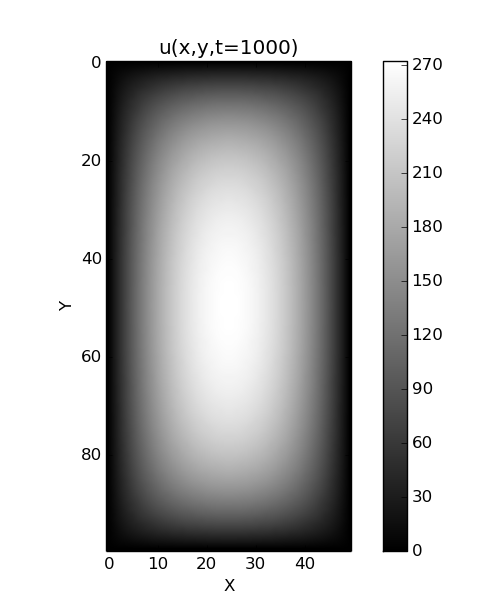
\includegraphics[width=0.5\textwidth]{purepython_res.png}
\caption{\label{FIG:purepython_res}Temperature distribution [Pure Python-solver]}
\end{figure}

\section*{5.2 Numpy and C implementations}
\subsection*{Numpy}
In stead of computing the terms one-by-one as done in 5.1, we can compute the whole 2D-matrix (called an array) at once and thus get rid of the loop over x and y-coordinate. This is done by vectorization of the code. One important thing to keep in mind, is that we want to exclude the boundary points. This means we have to pick out only the inner points and is done with the slice [1:-1,1:-1]. Note that we can use "comma" between the indices. Here we choose all x- and y-values starting from the second element and up to, but not included, the last one (index "-1"). When our update formula (\ref{EQ:upd_formula}), says $\pm$ 1 on an index, we have to move the entire slice the same. This can be seen in the code below:
\newline

\begin{minted}[bgcolor=LightGray, linenos, fontsize=\footnotesize]{python}
while t < t_end:
    u[1:-1,1:-1] = u[1:-1,1:-1] \
                 + dt*nu*(u[:-2,1:-1] + u[1:-1,:-2] - 4*u[1:-1,1:-1] \
                 +        u[1:-1,2:]  + u[2:,1:-1]) +nu*f[1:-1,1:-1]
    t += dt # Jump to next timestep
\end{minted}

Since the right hand side is computed and then assigned to the left hand side in one big step, we do not need a copy of the solution at the next time step, like we did before. Combined, these two changes saves computation time (drastically!) and halves the memory usage. Nice!

\subsection*{Results, NumPy}
The results is element wise exactly equal to the Python implementation, so no new figure is really needed (see fig.\ref{FIG:purepython_res}). However, the time spent computing is drastically lower, as we'll see later.

\subsection*{C, via Weave}
A third way to implement the time loop, is to use another language than Python, like C, and then do the heavy calculations here. Then we need some way to bridge these two languages, and my decision ended up on using Weave from the SciPy-package. We can then write C-code as a string, and call it with the \texttt{weave.inline()}-function. The time loop (and mesh grid loops) now look a lot like they did in the pure python-implementation, as can be seen below:
\newline

\begin{minted}[bgcolor=LightGray, linenos, fontsize=\footnotesize]{c}
int t,i,j;
for (t=0; t*dt<t_end+dt; t++){
    for (i=1; i<Nu[0]-1; i++) {
       for (j=1; j<Nu[1]-1; j++) {
           UN2(i,j) = U2(i,j) \
                    + dt*(U2(i-1,j) + U2(i,j-1) - 4*U2(i,j) \
                    + U2(i,j+1) + U2(i+1,j)) + nu*F2(i,j);
       }
    }
    for (i=1; i<Nu[0]-1; i++) {
       for (j=1; j<Nu[1]-1; j++) {
           U2(i,j) = UN2(i,j);
       }
    }
}
\end{minted}

The C-code above is stored as a string called \texttt{code} and is then executed with the following Python-code, where we have to tell what should be interpreted as constants, arrays etc, in a list of string-names. Weave then automatically makes some new variables we can use, like the dimensions n and m, is Nu[0] and Nu[1] (has nothing to do with $\nu$ / \texttt{nu}) and a 2D-array \texttt{u} is called \texttt{U2}. Indices is separated by a comma as in NumPy, but the brackets are curly. After computing \texttt{u\_new}, I copy these values to \texttt{u} through a double for-loop, to be used in the next iteration. This might seem slow, but as we'll see later, "for loops" in C are \textit{very} fast, so this is just fine!
\newline

\begin{minted}[bgcolor=LightGray, linenos, fontsize=\footnotesize]{python}
code = "int t,i,j; (.....)"
weave.inline(code, ['t_end','dt', 'u', 'un','f', 'nu'])
\end{minted}

\subsection*{Results, C via Weave}
As before, we get the exact same values computed (for all n-times-m-elements) and therefore I'd still like to refer the reader to figure \ref{FIG:purepython_res}. The advantage is of course even better performance in terms of speed, as we are going to examine in the next sections.



\end{document}


